\documentclass{article}

\usepackage{../preamble}
\standalonetrue

\title{MATH 316 Lecture 2}
\author{Ashtan Mistal}
\date{May 11 2021}

\begin{document}

\ifstandalone
\maketitle
\fi

\graphicspath{{./Lecture02/}}

\section{Solving the problem from last class}

We started with a simple example that was solvable using integrating factor, and we are now going to do the Taylor expansion of the \textbf{answer}, around the point $x = x_0$. THe confusion from last class was that we tried to solve the ODE using a Taylor expansion \textbf{of the differential equation}, as opposed to the actual answer. 

$$y(x) = y(0) + \frac{y'(0)}{1} x + \frac{y''(0)}{2!} x^2 + ...$$

$$y(x) = C \left[1 - x + \frac{3}{2} x^2 - \frac{7}{6} x^3 + ... \right]$$

From the class notes:

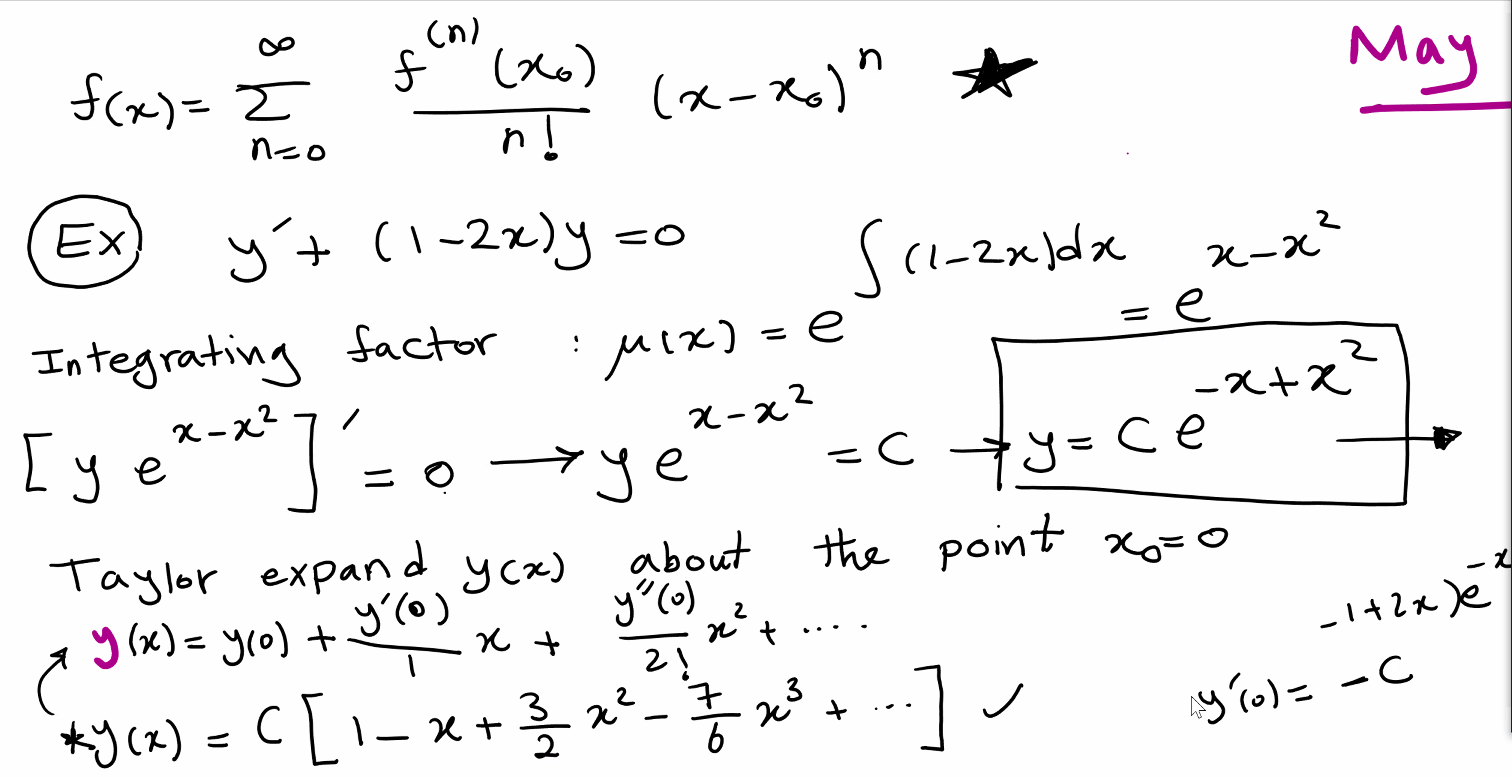
\includegraphics[width = 0.9 \textwidth]{image1.png}

Note that we factored C out of the taylor expansion. Moving forward, assume $y(x) = \sum_{n = 0}^{\infty} a_n x^n$. 

$$y' + (1 - 2x) y = 0$$

$$y' + y - 2xy = 0$$

$$\text{letting } y = \sum_{n = 0}^{\infty} a_n x^n, \text{ and } y' = \sum_{n = 1}^{\infty} a_n n x^{n-1}$$

$$\sum_{n = 1}^{\infty} a_n \underbrace{n}_{m = n-1; n = 1, m = 0} x^{n-1} + \sum_{n = 0}^{\infty} \underbrace{a_n}_{m = n} x^n - 2 \sum_{n = 0}^{\infty} \underbrace{a_n}_{m = n+1;  n = 0, m = 1} x^{n+1} = 0$$

Not exactly sure what these variables are doing with the $n$ and $m$... I guess they're dummy variables that we're using for each sum. 

$$ \sum_{m = 0}^{\infty} a_{m+1} (m+1)x^m + \sum_{m = 0}^{\infty} a_m x^m - 2 \sum_{m = 1}^{\infty} a_{m-1} x^m = 0$$

Peel-off:

$$a_1 x^0 + a_0 x^0 + \sum_{m = 1}^{\infty} \left[a_{m+1} (m+1) + a_m - 2 a_{m-1} \right] x^m = 0$$

Note that $x^0, x, x^2, ..., x^n$ are linearly independent. 

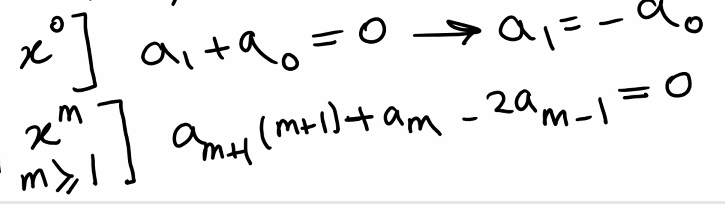
\includegraphics[width = 0.7 \textwidth]{image2.png}

Q: Why do we need to shift the indices?

A: We want to get to a single sigma -- A single sum. If we don't do it, we aren't able to get to a single relation. Indices must start at the same point to be able to combine sums. 

From the relation $a_{m=1} (m+1) + a_m - 2 a_{m-1} = 0$, we can find the relation:

$$a_{m+1} = \frac{-a_m + 2 a_{m-1}}{m+1}$$

$$m = 1: a_2 = \frac{-a_1 + 2 a_0}{2} = \frac{3}{2} a_0$$

$$m = 2: a_3 = \frac{-a_2 + 2 a_1}{3} = \frac{-7}{6} a_0$$

$$y(x) = a_0 + a_1 x + a_2 x^2 + a_3 x^3 + ...$$

$$ y(x) = a_0 - a_0 x + \frac{3}{2} a_0 x^2 - \frac{7}{6} a_0 x^3 + ...$$

$$y(x) = a_0 \left[ 1 - x + \frac{3}{2} x^2 - \frac{7}{6} x^3 + ... 
\right]$$

$$ = \text{Taylor expansion of the direct solution}$$

\section{Example 2}

$$ x y' + (2 - x) y = 0$$

$$ y' + \frac{2-x}{x} y = 0$$

Solving this using integrating factor method, we find the following:

$$\mu(x) = e^{\int \frac{1-x}{x} dx} = e^{2 \ln x - x} = x^2 e^{-x}$$

$$\left[x^2 e^{-x} y \right]' = 0 \rightarrow y = \frac{C}{x^2 e^{-x}} = C x^-2 e^x$$

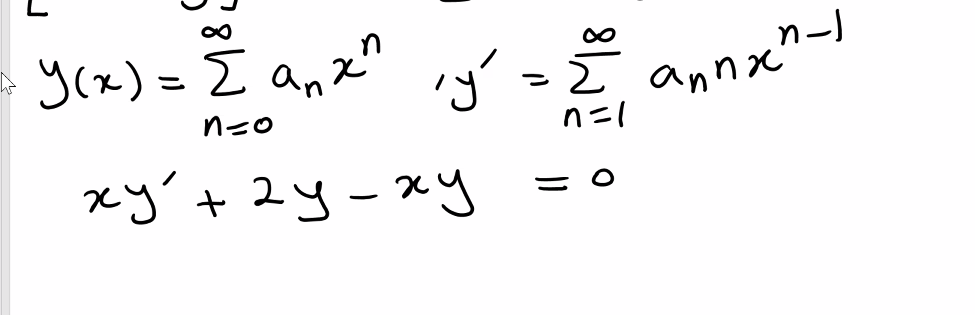
\includegraphics[width = 0.9 \textwidth]{image3.png}

$$\sum_{n = 1}^{\infty} a_n n x^n + 2 \sum_{n = 0}^{\infty} a_n x^n - \sum_{n = 0}^{\infty} a_n x^n+1 = 0$$

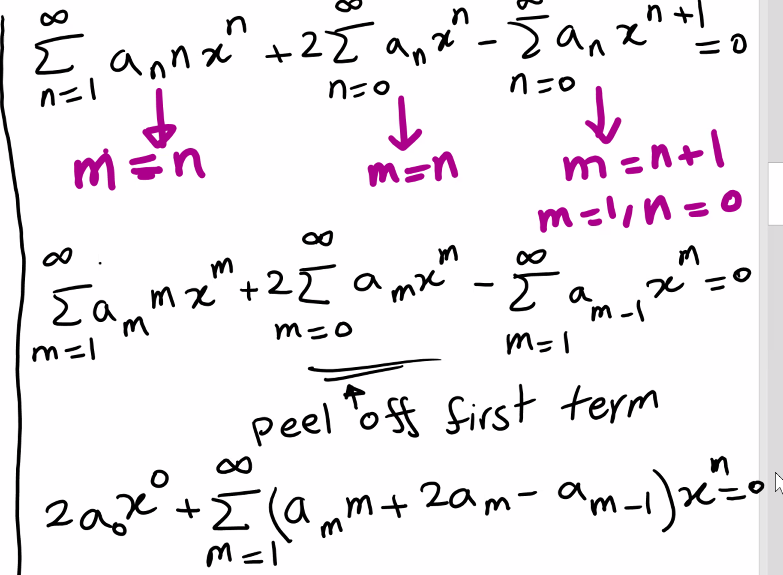
\includegraphics[width = 0.9 \textwidth]{image4.png}

$$\left. x^0 \right] 2 a_0 = 0 \longrightarrow a_0 = 0$$

$$ \left. \begin{matrix} x^m \\ m \geq 1 \end{matrix} \right] a_m (m+2) = a_{m-1}$$

$$\text{note that } a_m = \frac{a_{m-1}}{m+2} \text{for m} \geq 1$$

$$m = 1: a_1 = \frac{a_0}{3} = 0$$

$$m = 2: a_2 = \frac{a_4}{4} = 0$$

This is a trivial solution; they are all zero (and will continue to be). 

$y = c x^{-2} e^x$ is the general solution. 

$$ = C \underbrace{x^{-2}}_{\text{Capture the singularity}} \underbrace{\left[ 1 + x + \frac{x^2}{2!} + \frac{x^3}{3!} + ... \right]}_{\sum_{n = 0}^{\infty} a_n x^n}$$

$$ y(x) = \underbrace{x^r}_{\text{Capture singularity}} \sum_{n = 0}^{\infty} a_n x^n$$

This brings us to the \textbf{Frobenius Series}. 

\section{Frobenius Series}

Let's define ordinary \& singular points:

A linear 2nd order ODE:

$$P(x) y'' + Q(x) y' + r(x) y = 0$$

$$y'' + \frac{Q(x)}{P(x)} y' + \frac{R(x)}{P(x)} y = 0$$

Letting $p(x) = \frac{Q(x)}{P(x)}$ and $q(x) = \frac{R(x)}{P(x)}$. If they are both \textbf{analytic} at the point $x_0$. i.e. they have Taylor expansions about $x_0$, $x_0$ is an ordinary point. Otherwise, $x_0$ is a singular point. 

Example: $\left. \begin{matrix} p(x) = \frac{1}{x} \\ p(x) = \ln(x) \end{matrix} \right\} \text{At } x = 0 \text{, not analytic}$.

Analytic means that is is expressible as a power series around $x_0$. It means that it is infinitely differentiable around $x_0$. 

\subsubsection{Quick notes}

\begin{itemize}
    \item A power series solution is possible for all ordinary points (similar to the first example we saw), but not all singular points. 
    \item For singular points, we introduce the Frobenius Series. However, this only works for some singular points. 
    \item Singular points results in the change of the nature of the ODE. Ordinary points exists in the domain of $p(x)$ and $q(x)$. 
    \item The radius of convergence of the power series is at least as large as the distance from the $x_0$ to the nearest singular point.
    \begin{itemize}
        \item For example, when we had $y = C x^{-2} e^x$, we realize that $x=  0$ is a singular point. 
        \item We can see this in both the answer as well as the ODE. \item When we plot the function, it looks like this:
        \item 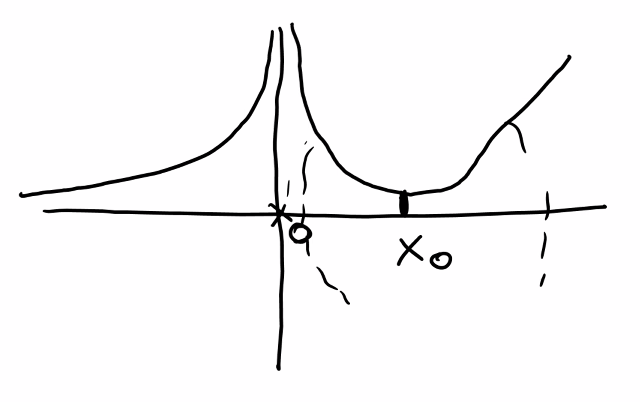
\includegraphics[width = 0.5 \textwidth]{image6.png}
        \item The dotted circles around $x_0$ is the radius of convergence. 
    \end{itemize}
\end{itemize}

Example:

$$y' + (1 - 2x)y =0$$

$$y(x) = C e^{-x + x^2}$$

There are no singular points. Hence the radius of convergence is infinity. 

\subsection{Singular Points}

Singular points are divided into two classes:

\begin{itemize}
    \item Regular singular points, that we use the Frobenius series solution for
    \item Irregular singular points (Beyond this course). For these, we \textbf{cannot} use Frobenius series. 
\end{itemize}

\end{document}
